%pdflatex abra.tex
%convert -density 150x150 abra.pdf abra.png
% white background
%convert -density 150x150 -background white -alpha remove -alpha off abra.pdf abra.png
\documentclass[border={2pt 2pt 2pt 2pt}]{standalone}
\usepackage{tikz}
\usetikzlibrary{calc}
\begin{document}

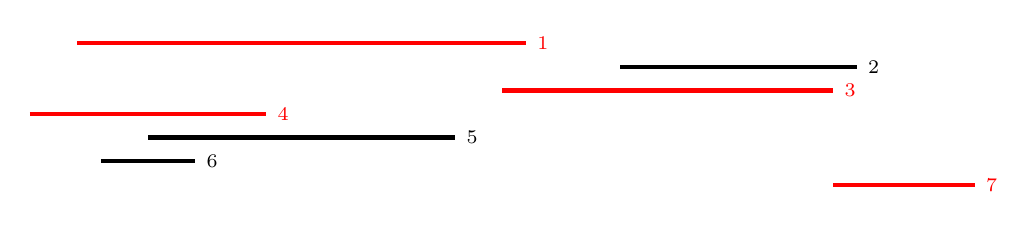
\begin{tikzpicture}[scale=0.3]
\coordinate (A1) at (2,0);
\coordinate (A2) at (21,0);
\coordinate (B1) at (25,-1);
\coordinate (B2) at (35,-1);
\coordinate (C1) at (20,-2);
\coordinate (C2) at (34,-2);
\coordinate (D1) at (0,-3);
\coordinate (D2) at (10,-3);
\coordinate (E1) at (5,-4);
\coordinate (E2) at (18,-4);
\coordinate (F1) at (3,-5);
\coordinate (F2) at (7,-5);
\coordinate (G1) at (34,-6);
\coordinate (G2) at (40,-6);
\draw[red,ultra thick] (A1)--(A2)node[right]{\scriptsize 1};
\draw[ultra thick] (B1)--(B2)node[right]{\scriptsize 2};
\draw[red,ultra thick] (C1)--(C2)node[right]{\scriptsize 3};
\draw[red,ultra thick] (D1)--(D2)node[right]{\scriptsize 4};
\draw[ultra thick] (E1)--(E2)node[right]{\scriptsize 5};
\draw[ultra thick] (F1)--(F2)node[right]{\scriptsize 6};
\draw[red,ultra thick] (G1)--(G2)node[right]{\scriptsize 7};
%\draw[blue,very thick,fill=white] (A) circle [radius=0.5];
%\node at (A) {\huge\bf 1};
\end{tikzpicture}

\end{document}
